\section{Codework}

In order to solve the thermoacoustic governing equations, these 4 method could be programmed to get parametric and quick results. 

JULIA programming language is preferred to perform codeworks.

\subsection{Why Julia Programming Language?}

Julia programming language is developed in order to perform matrix calculations reasonably fast and easy. It is completely open source programming language which enables to work without getting licence. Additionally, having high-level programming syntax makes it easy to learn and its computing performance is blazing fast comparing to programming languages like MATLAB and Python. Furthermore, dynamic type syntax is not requiring to define parameter type(\textit{int, float, double, string, char}) such as fast programming languages C++ and Fortran. 

\subsection{Programming Methodology}

During the code development, mathematical model is created based on object oriented programming technique. Followed methodology is illustrated in Figure \ref{fig:flowchart}. 

\FloatBarrier
\begin{figure}[!t]
	
	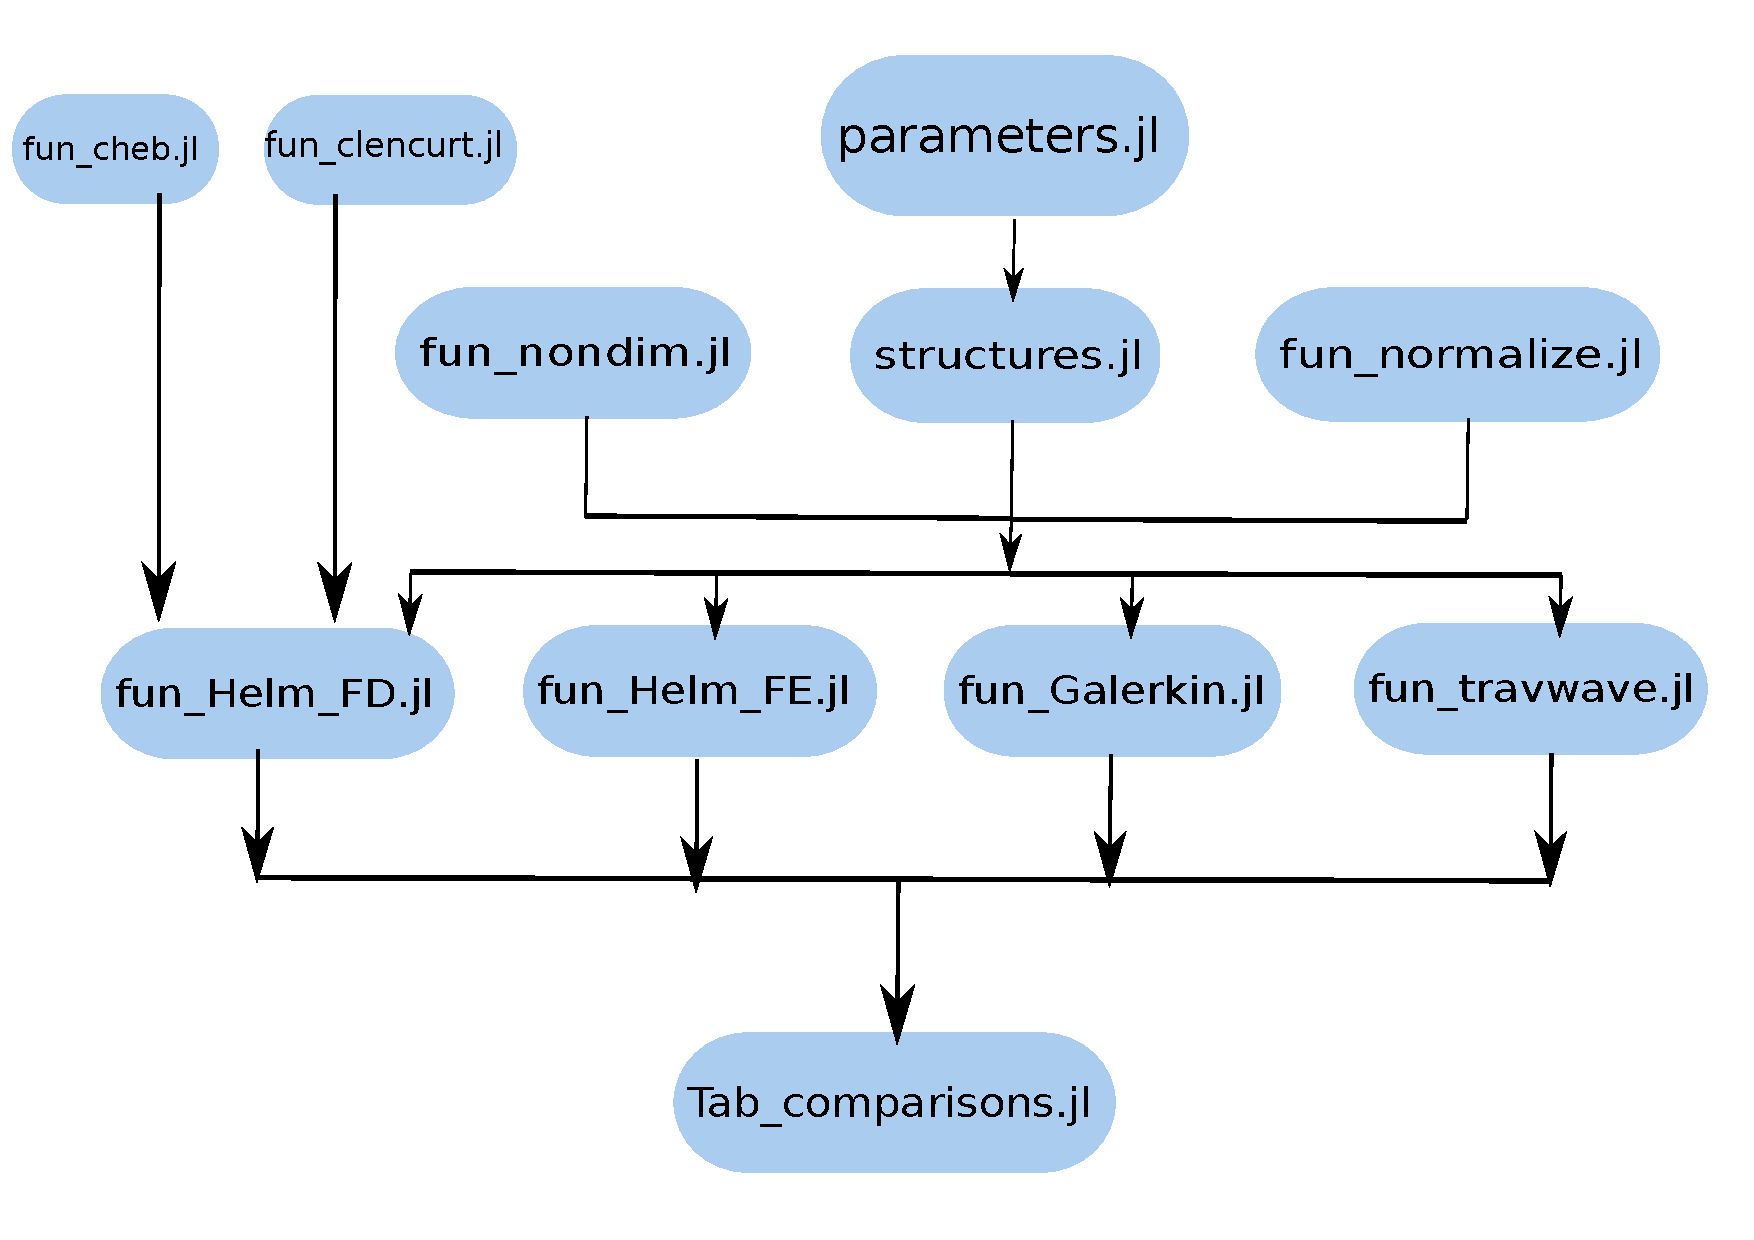
\includegraphics[width=\textwidth]{flowchart.pdf}
	\caption{Codework layout and proposed flowchart}
	\label{fig:flowchart}
	
\end{figure}
\FloatBarrier

Figure \ref{fig:flowchart} shows that each Julia file is connected by following systematic approach. By using these codes, all the methods' calculations can be performed and obtained results and table can be generated in file \textit{Tab\_comparisons.jl}. Script \textit{structures.jl} includes structures of \textbf{emode} and \textbf{ds}. These 2 structures are determined and returned by 4 main scripts;\textit{fun\_Helm\_FD.jl}, \textit{fun\_Helm\_FE.jl}, \textit{fun\_Galerkin.jl and \textit{fun\_travwave.jl}} Specified model parameters are inserted into \textit{parameters.jl} file. Moreover, normalization and non-dimensionalization are performed by \textit{fun\_normalize.jl} and \textit{fun\_nondim.jl} files respectively.
